\section{实验结果展示}
\subsection{客户端和服务器端的初始界面}
运行客户和服务器两个工程,我们便得到了初始界面,如下:
\begin{figure}[H]
  \centering
  % Requires \usepackage{graphicx}
  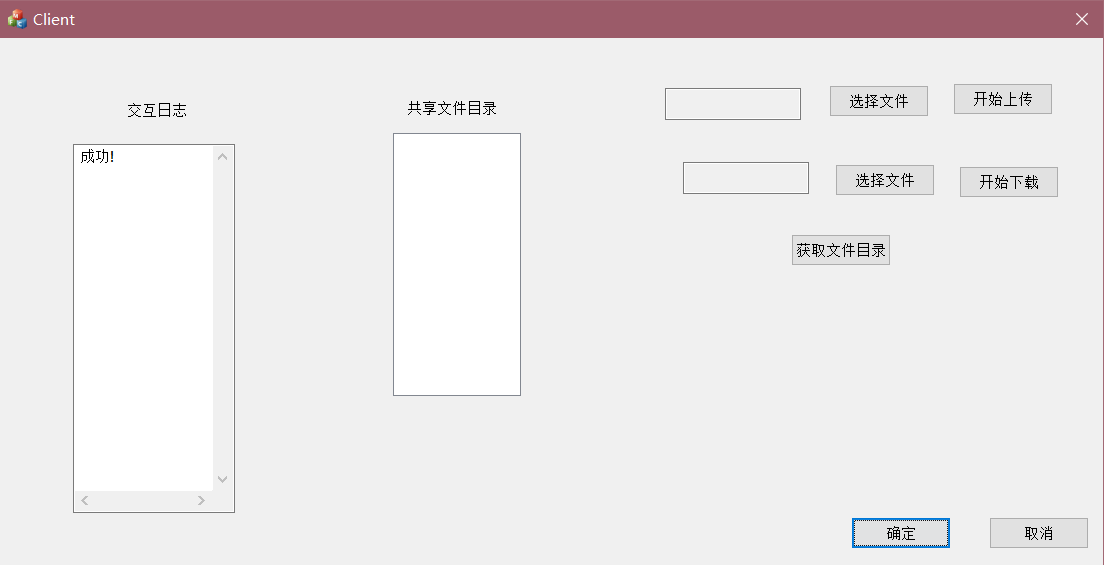
\includegraphics[width=0.8\linewidth]{figure/client_init}\\
  \caption{客户端初始界面}
\end{figure}

\begin{figure}[H]
  \centering
  % Requires \usepackage{graphicx}
  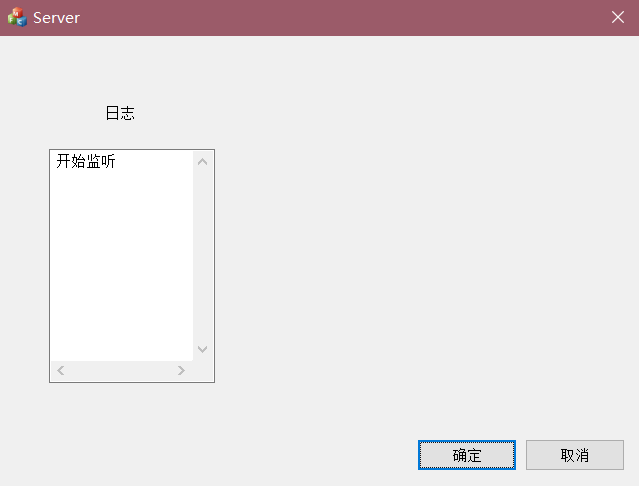
\includegraphics[width=0.8\linewidth]{figure/server_init}\\
  \caption{服务器端端初始界面}
\end{figure}

\subsection{共享目录的获取}
我们在客户端点击获取共享目录按钮,便可以获得服务器端的共享目录,两端变化如下:

\begin{figure}[H]
  \centering
  % Requires \usepackage{graphicx}
  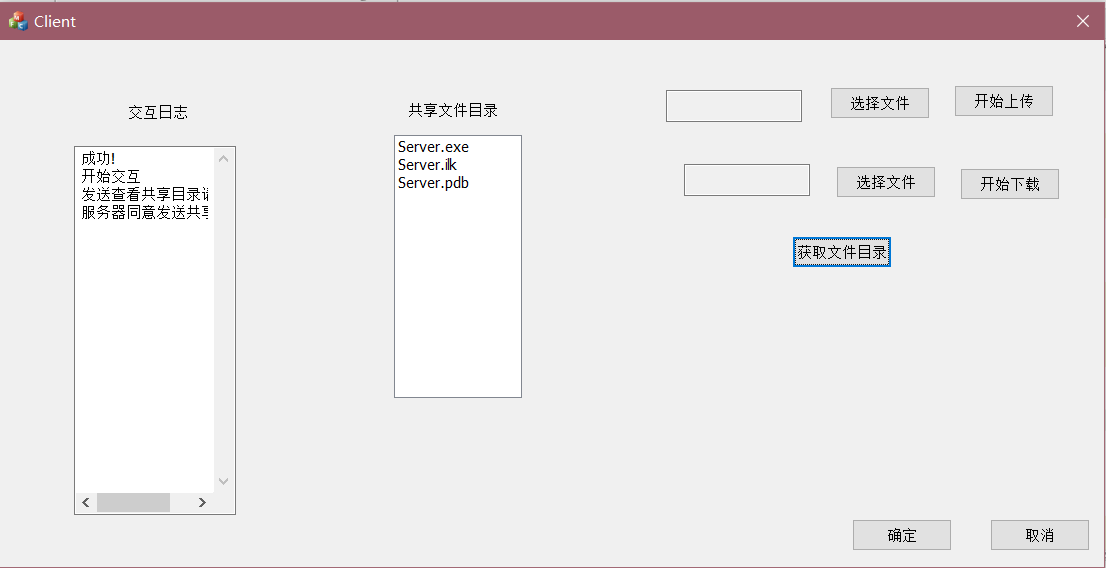
\includegraphics[width=0.8\linewidth]{figure/client_file_dic}\\
  \caption{客户端获取共享目录}
\end{figure}

\begin{figure}[H]
  \centering
  % Requires \usepackage{graphicx}
  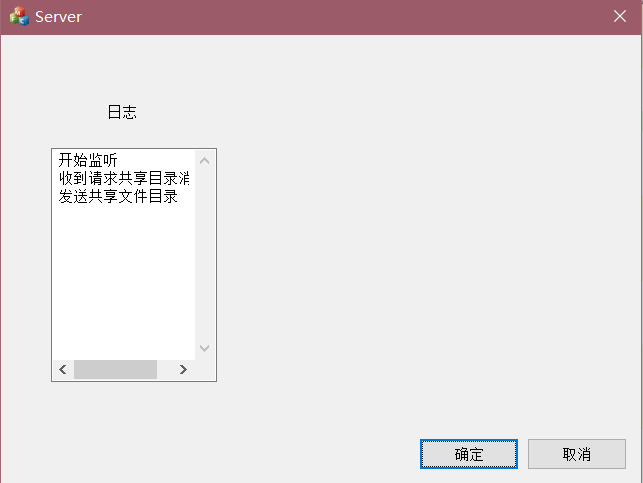
\includegraphics[width=0.8\linewidth]{figure/server_file_dic}\\
  \caption{服务器端获取共享目录}
\end{figure}

\subsection{客户端上传文件}
我们选择上传文件后点击“开始上传”按钮,我们便可以进行文件的上传了
\begin{figure}[H]
  \centering
  % Requires \usepackage{graphicx}
  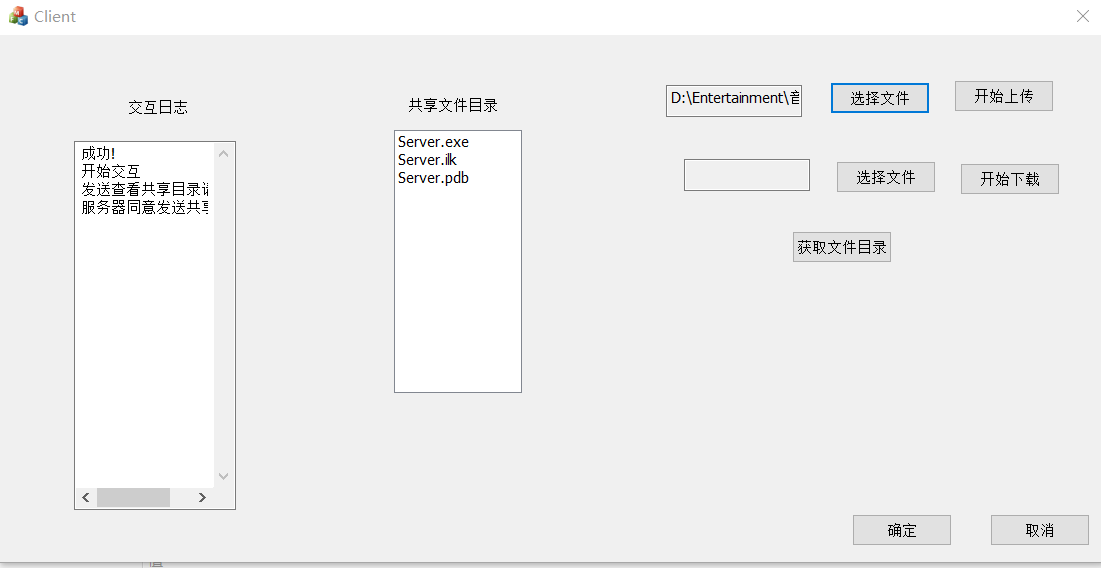
\includegraphics[width=0.8\linewidth]{figure/client_before_upload}\\
  \caption{客户端上传前}
\end{figure}
\begin{figure}[H]
  \centering
  % Requires \usepackage{graphicx}
  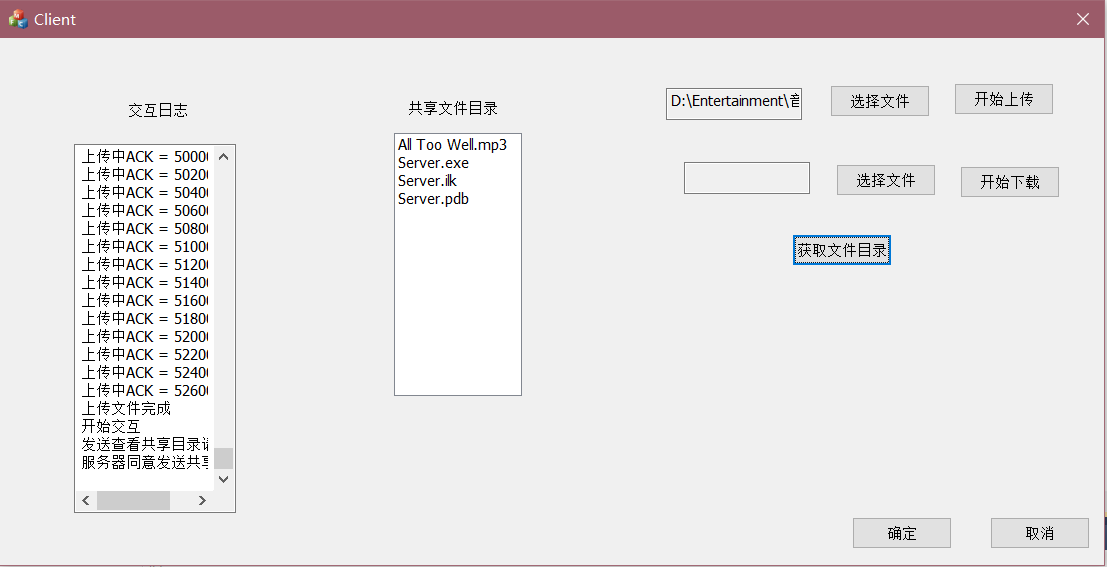
\includegraphics[width=0.8\linewidth]{figure/client_after_upload}\\
  \caption{客户端上传完成}
\end{figure}


\begin{figure}[H]
  \centering
  % Requires \usepackage{graphicx}
  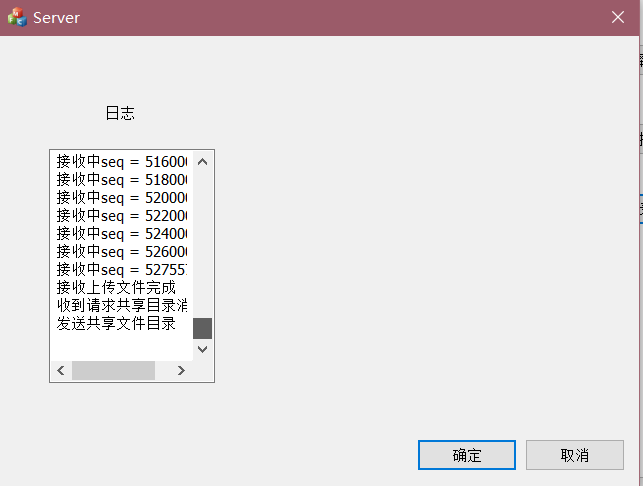
\includegraphics[width=0.8\linewidth]{figure/server_upload}\\
  \caption{服务器端接收上传完成}
\end{figure}
可以看到,共享目录增加了上传的文件,实验成功。

\subsection{客户端下载文件}
我们在客户端的共享目录中选择要下载的文件,然后点击“开始下载”按钮后,我们便可以进行文件的下载了。
\begin{figure}[H]
  \centering
  % Requires \usepackage{graphicx}
  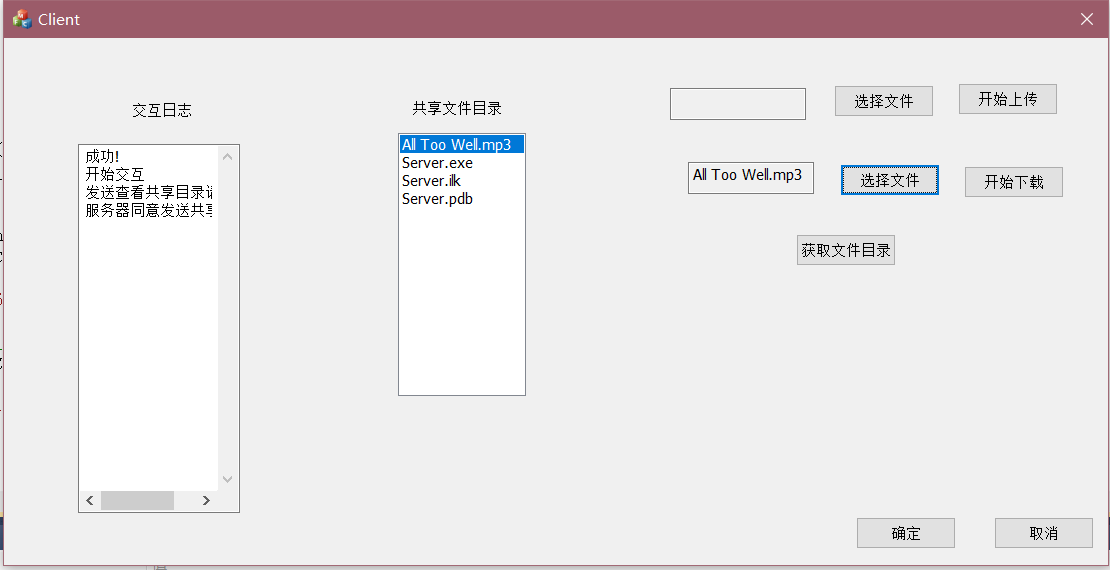
\includegraphics[width=0.8\linewidth]{figure/client_before_download}\\
  \caption{客户端下载前}
\end{figure}
\begin{figure}[H]
  \centering
  % Requires \usepackage{graphicx}
  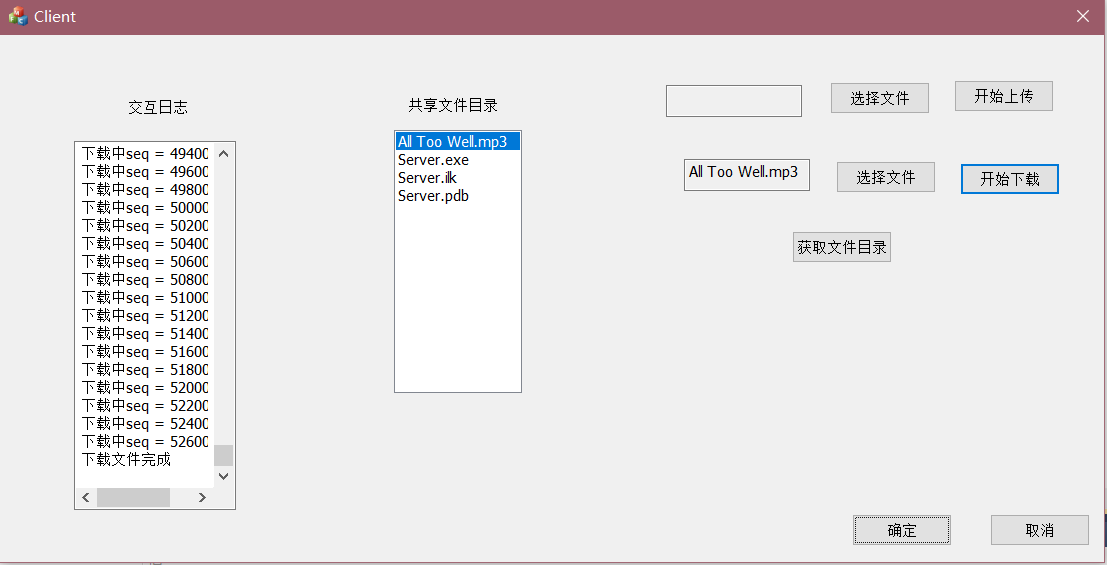
\includegraphics[width=0.8\linewidth]{figure/client_after_download}\\
  \caption{客户端下载完成后}
\end{figure}
\begin{figure}[H]
  \centering
  % Requires \usepackage{graphicx}
  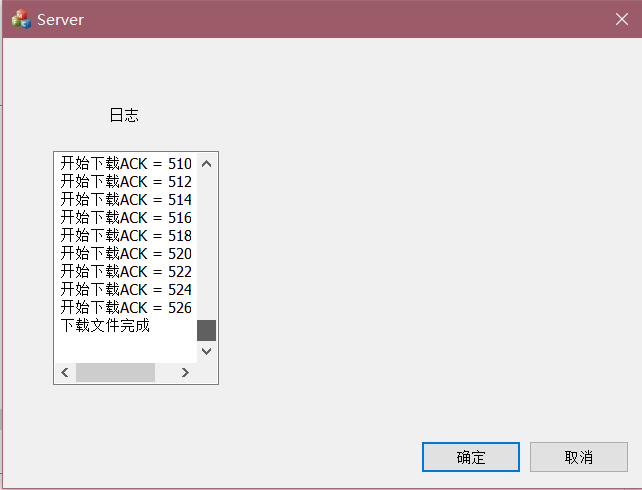
\includegraphics[width=0.8\linewidth]{figure/server_download}\\
  \caption{服务器端下载完成后}
\end{figure}

我们在客户端文件夹中可以看到获取了正确的文件,实验成功。

\subsection{多用户}

\begin{figure}[H]
  \centering
  % Requires \usepackage{graphicx}
  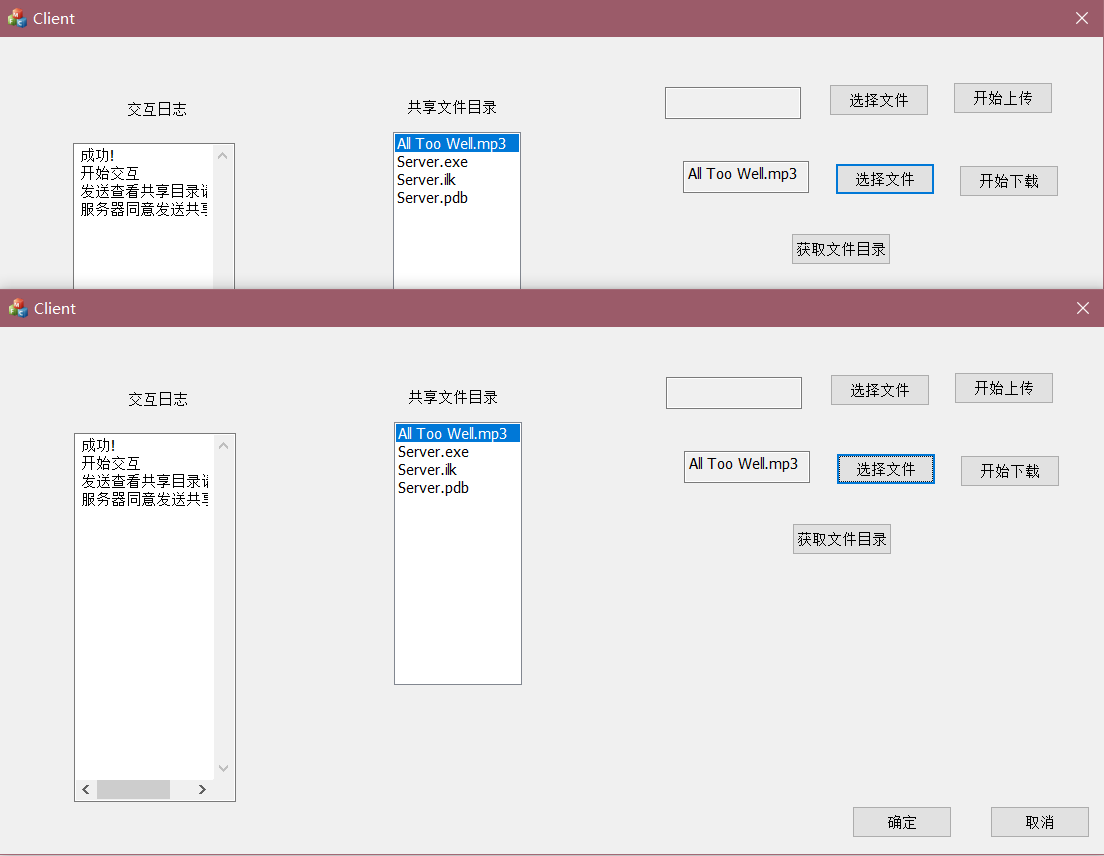
\includegraphics[width=0.8\linewidth]{figure/multiclient_before_download}\\
  \caption{多用户下载前}
\end{figure}
\begin{figure}[H]
  \centering
  % Requires \usepackage{graphicx}
  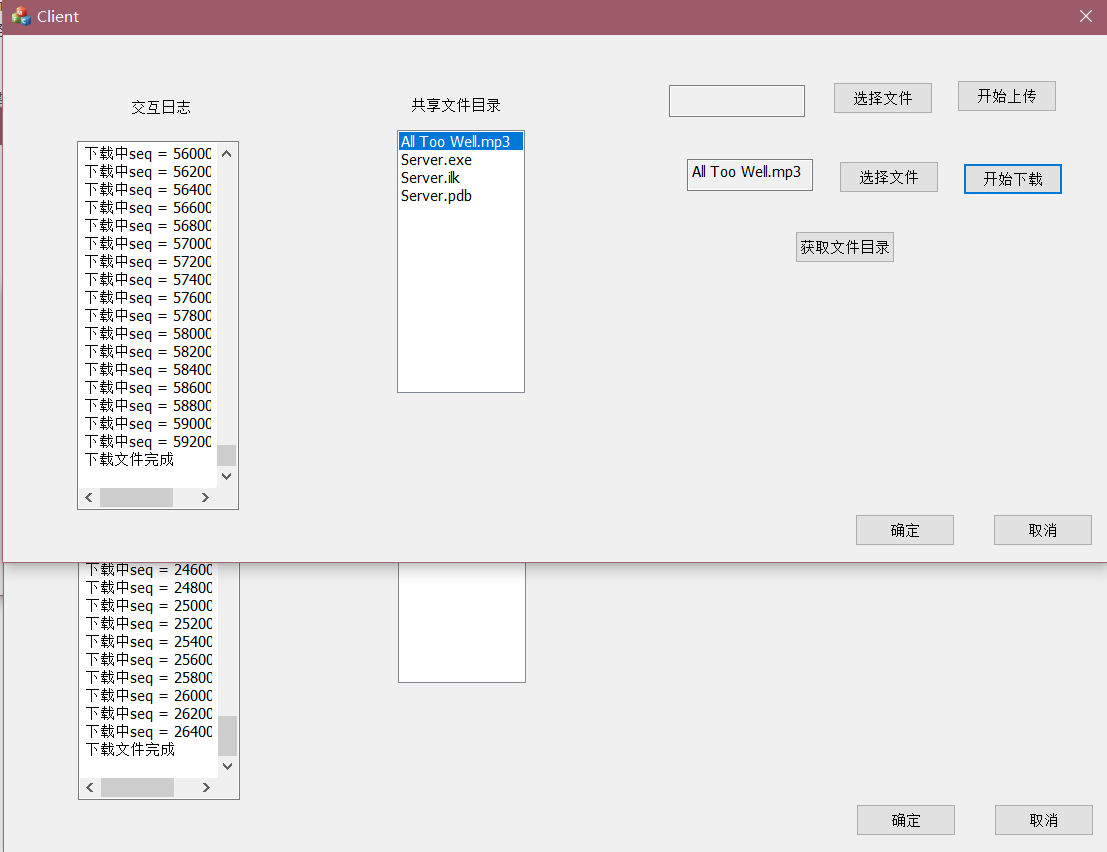
\includegraphics[width=0.8\linewidth]{figure/multiclient_after_download}\\
  \caption{多用户下载完成后}
\end{figure}
\begin{figure}[H]
  \centering
  % Requires \usepackage{graphicx}
  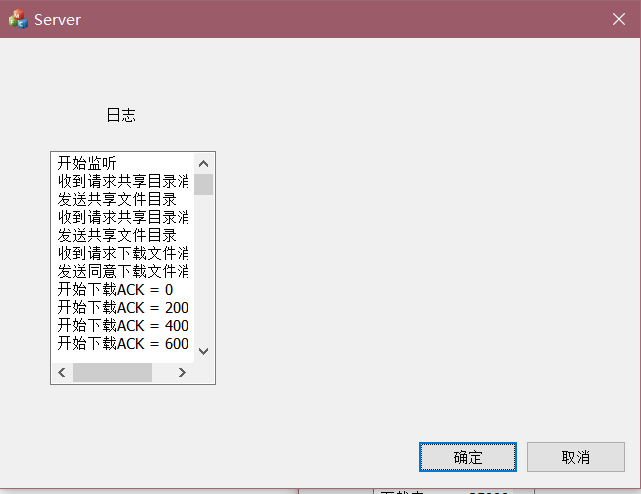
\includegraphics[width=0.8\linewidth]{figure/multiserver_download}\\
  \caption{多用户服务器端下载完成后}
\end{figure}

可以看到在服务器端显示了两条下载完成记录,两个客户端也正确完成了下载。
\clearpage
